\chapter{Výsledky a diskuse}
Kapitola shrnuje a interpretuje výsledky parametrizací metod EEM a PEOE za užití navržených klasifikací atomů s cílem zhodnotit, zda jsou pro parametrizaci postačující základní klasifikace atomů nebo je pro tento problém vhodné aplikovat detailnější dělení. Veškeré výsledky parametrizací lze nalézt v externí příloze bakalářské práce nebo na adrese \url{https://lcc.ncbr.muni.cz/~raduse19/}.  

\section{Vstupní data}
Pro parametrizaci empirických metod byly použita molekulová sada CCD\_gen a sada Protein. Pro analýzu přenositelnosti parametrů byly molekuly v molekulových sadách rozděleny na sadu tréninkovou a validační v poměru 9:1. Software MACH zajistil, aby validační sada vždy obsahovala identické atomové typy jako sada tréninková. Empirické metody byly pro obě molekulové sady parametrizovány vůči referenčním nábojům typu B3LYP/6-311G*/NPA.
% Klasifikace určené pro formát SDF byly nejdříve zkušebně aplikovány na tréninkovou sadu obsahující 500 molekul a použity pro parametrizaci. 
\begin{table}[h]
    \renewcommand{\arraystretch}{1.35}
    \centering
    \begin{tabular}{l|l|l}
         sada molekul &  \textbf{CCD\_gen}\footnotemark
         & \textbf{Protein}\\
         \hline
         počet molekul & 4 443 & 32\\
         počet atomů & 204 760 & 29 107\\
         počet atomů v molekule & 3-305 & 166-1 174 \\
         zdroj struktur & software CORINA & RTG krystalografie \\
         \hline
         \multirow{2}{8em}{molekuly} & 
            ligandy z databáze PDB & malé proteiny\\
         & pouze validní struktury & \makecell[l]{neobsahuje ligandy ani \\nestandardní residua}
    \end{tabular}
    \caption{Souhrn informací o molekulových sadách užitých pro parametrizaci. Molekuly obou sad byly doplněny o vodíky a byla optimalizována jejich geometrie.}
    \label{moleculesets}
\end{table}
\footnotetext{ zdroj: RAČEK, T., PAZÚRIKOVÁ, J., SVOBODOVÁ VAŘEKOVÁ, R. et al. „NEEMP: software for validation, accurate calculation and fast parameterization of EEM charges“. \textit{Journal of Cheminformatics}. 2016, \textbf{8}(1). DOI: 10.1186/s13321-016-0171-1.}
% \makecell[l]{malé proteiny bez ligandů\\a nestandarních residuí}\\
\section{Výsledky parametrizace}
Pro popis výsledků parametrizací empirických metod za užití různých klasifikátorů je zavedeno značení 'molekulová sada/empirická metoda/užitý klasifikátor'. Výpočty  parametrizací probíhaly na serverech virtuální organizace MetaCentrum. 

Klasifikátory \verb|hbo|, \verb|hybrid|, \verb|substruct| a \verb|peptide| se po vyhodnocení statistik a korelačních grafů prokázaly pro parametrizaci metod EEM a PEOE jako platné. 
%markantní rozdíly byly nalezeny zejména v čase výpočtu jednotlivých parametrizací.
%Výsledky všech parametrizací používajících implementované klasifikátory jsou srovnávány s referenčním klasifikátorem \verb|plain|, který dělí atomy do atomových typů dle  protonového čísla. 
Pro každý implementovaný klasifikátor je výsledek dané parametrizace srovnán s parametrizací využívající klasifikaci atomů dle protonového čísla. Referenční klasifikátor je označen jako \verb|plain| a je implementován v softwaru MACH. Klasifikátor \verb|partners| generuje pro obsáhlé molekulové sady extrémní množství atomových typů (pro sadu CCD\_gen konkrétně 235), jeho použití proto nelze obecně doporučit. 


PCC$^2$ získaných empirických a referenčních nábojů nabývá napříč parametrizacemi minimální hodnoty 0,9781 pro SDF/EEM/hybrid parametrizaci, hodnota RMSD je maximálně 0,0623, a to u téže parametrizace. Statistiky parametrizací sady CCD\_gen lze nalézt v následující tabulce \ref{statistics}. Statistiky parametrizací sady Protein jsou umístěny v~\hyperref[proteinstat]{příloze}. 
\medskip
\begin{table}[h]
    \renewcommand{\arraystretch}{1.4}
    \centering
    \begin{tabular}{c|l|l|l|l|l|l}
         \textbf{klasifikátor} &  \textbf{metoda} & \textbf{RMSD} & \textbf{PCC$^2$} & \textbf{MAE} & \textbf{ABSMAX} & \textbf{doba výpočtu}\\
         \hline
         \multirow{2}{6em}{\texttt{hbo}} & EEM & 0,0582 & 0,9809 & 0,0405 & 0,7133 & 1:59:29  \\
         & PEOE & 0,0394 & 0,9912 & 0,0259 & 0,7313 & 2:53:04 \\
         \hline
         \multirow{2}{6em}{\texttt{hybrid}} & EEM & 0,0620 & 0,9781 & 0,0424 & 0,7475 & 1:15:40 \\
         & PEOE & 0,0479 & 0,9870 & 0,0310 & 1,0619 & 1:42:28 \\
         \hline
         \multirow{2}{6em}{\texttt{substruct}} & EEM & 0,0479 & 0,9870 & 0,0300 & 0,6593 & 17:46:49 \\
         & PEOE & 0,0464 & 0,9878 & 0,0293 & 0,9175 & 6:56:11 \\
         \hline
         \multirow{2}{6em}{\texttt{plain}} & EEM & 0,0000 & 0,0000 & 0,0000 & 0,0000 & 17:46:49 \\
         & PEOE & 0,0000 & 0,0000 & 0,0000 & 0,0000 & 6:56:11
    \end{tabular}
    \caption{Výsledky vybraných statistik parametrizace sady SDF. Jsou zaznamenány pouze statistiky tréninkových sad.}
    \label{statistics}
\end{table}
\medskip

Hodnota PCC$^2$ napříč parametrizacemi za užití SDF i PDB sady neklesá pod hodnotu 0,97; lze tedy vyvodit, že náboje atomů získané skrze parametrizace silně lineárně korelují s referenčními náboji (viz obr. \ref{graph_corr_EEM}). Hodnoty RMSD pro vypočtené empirické a~referenční náboje se pohybují nejčastěji v rozmezí 0,040-0,055; u PDB sady v některých případech klesají až k hodnotě 0,023. Uvedená rozmezí hodnot statistik platí jak pro tréninkové, tak validační sady molekul. 

Rozdíl hodnot RMSD tréninkových a validačních sad je nejčastěji v řádu desetitisícin, maximální hodnota tohoto rozdílu je 0,018. Hodnot PCC$^2$ zmíněných sad se liší v~řádu tisícin či desetitisícin, pro MAE a ABSMAX rozdíl proniká až do řádu setin. Na základě těchto údajů lze  parametry získané užitím implementovaných klasifikátorů pokládat za přenositelné.

\begin{table}[h]
    \renewcommand{\arraystretch}{1.4}
    \centering
    \begin{tabular}{c|l|l|l|l|l}
         \textbf{metoda} & \textbf{sada} & \textbf{RMSD} & \textbf{PCC$^2$} & \textbf{MAE} & \textbf{ABSMAX}\\
         \hline
         \multirow{2}{4em}{EEM} & train & 0,0582 & 0,9809 & 0.0405 & 0,7133  \\
         & test & 0,0566 & 0,9819 & 0,0397 & 0,7045 \\
         \hline
         \multirow{2}{4em}{PEOE} & train & 0,0394 & 0,9912 & 0.0259 & 0,7313  \\
         & test & 0,0386  & 0,9916 & 0,0258 & 0,4765 \\
    \end{tabular}
    \caption{Porovnání statistik tréninkových a validačních sad klasifikátoru \texttt{hbo}. Statistiky se vztahují ke klasifikaci SDF molekulové sady.}
    \label{prenositelnost}
\end{table}
\vspace{2cm}
% Náboje atomů v molekulové sadě získané skrze parametrizace pro každý výpočet silně lineárně korelují s náboji sady validační. Hodnoty RMSD parciálních atomových nábojů vypočtených na tréninkové a validační sadě se napříč parametrizacemi liší nejvíce o 0,0018. 

% - nejvýraznější rozdíly ve statistikách + čas výpočtu (závislost na škálování metody)
% - trend: PEOE náboje - linearizace pro jednotlivé atomové typy + důvod 

Z korelačních grafů empirických a referenčních nábojů je patrné, že metoda PEOE přiřazuje v určitých případech atomům náboje o konstatní hodnotě, což v grafu odpovídá vodorovným shlukům bodů. Přiřazení konstaních či velmi podobných hodnot parciálních nábojů vyplývá z iterativního způsobu výpočtu. Metoda PEOE navíc pracuje pouze s~topologií molekuly a atomům, které mají stejné chemické okolí, implicitně přiřazuje stejné náboje (viz obr. \ref{graph_corr_PEOE} nebo příloha [ref]).

\subsection{Úprava klasifikátorů 'substruct' a 'peptide'}
Časová náročnost parametrizací za použití klasifikátorů \verb|substruct| a \verb|peptide| se v porovnání s ostatními klasifikátory ukázala jako netriviální z důvodu velkého množství definovaných atomových typů. Po analýze korelačních grafů byly vybrané atomové typy sloučeny, počet atomových typů byl u obou klasifikátorů zredukován přibližně na polovinu.

\begin{table}[h]
    \renewcommand{\arraystretch}{1.4}
    \centering
    \begin{tabular}{c|l|l|l|l|l|l}
         \textbf{klasifikátor} &  \textbf{metoda} & \textbf{RMSD} & \textbf{PCC$^2$} & \textbf{MAE} & \textbf{ABSMAX} & \textbf{doba výpočtu}\\
         \hline
         \multirow{2}{6em}{\texttt{substruct}} & EEM & 0,0334 & 0,9948 & 0,0229 & 0,3880 & 23:01:14  \\
         & PEOE & 0,0493 & 0,9887 & 0,0292 & 0,4484 & 0:19:51 \\
         \hline
         \multirow{2}{6em}{\texttt{substruct simplified}} & EEM & 0,0388 & 0,9930 & 0,0265 & 0,3198 & 14:30:45 \\
         & PEOE & 0,0514 & 0,9876 & 0,0319 & 0,5083 & 0:13:02 \\
         \hline
         \multirow{2}{6em}{\texttt{peptide}} & EEM & 0,0359 & 0,9940 & 0,0228 & 0,3558 & 1 den, 15:03:35 \\
         & PEOE & 0,0456 & 0,9902 & 0,0293 & 0,3147 & 0:29:01 \\
         \hline
         \multirow{2}{6em}{\texttt{peptide simplified}} & EEM & 0,0389 & 0,9929 & 0,0266 & 0,3647 & 18:28:26 \\
         & PEOE & 0,0512 & 0,9877 & 0,0302 & 0,2536 & 0:15:12
    \end{tabular}
    \caption{Srovnání statistik původních a zjednodušených klasifikátorů \texttt{peptide} a~\texttt{substruct} aplikovaných na PDB sadě. V tabulce jsou zaznamenány pouze statistiky tréninkových sad.}
    \label{statistics_simplified}
\end{table}

Statistiky zjednodušených klasifikací se od statistik původních klasifikátorů liší pou\-ze minimálně, rozdíly hodnot jednotlivých statistik se týkají řádu tisícin, ve výjimečných případech setin. Zjednodušením klasifikace se docílilo snížení časové náročnosti parametrizace zhruba na polovinu, a to s minimálním vlivem na kvalitu vypočtených parametrů.

%Výsledky redukce atomových typů klasifikátorů \verb|substruct| a \verb|peptide| potvrdily hypotézu, že klasifikace atomů s menším množstvím definovaných atomových typů jsou pro účely parametrizace z výpočetního hlediska vhodnější než detailní klasifikace, přičemž statistiky empirických a referenčních nábojů zůstávají při zavedení méně detailních klasifikací oproti podrobným klasifikacím téměř nezměněny.

\begin{figure}[]
\begin{center}
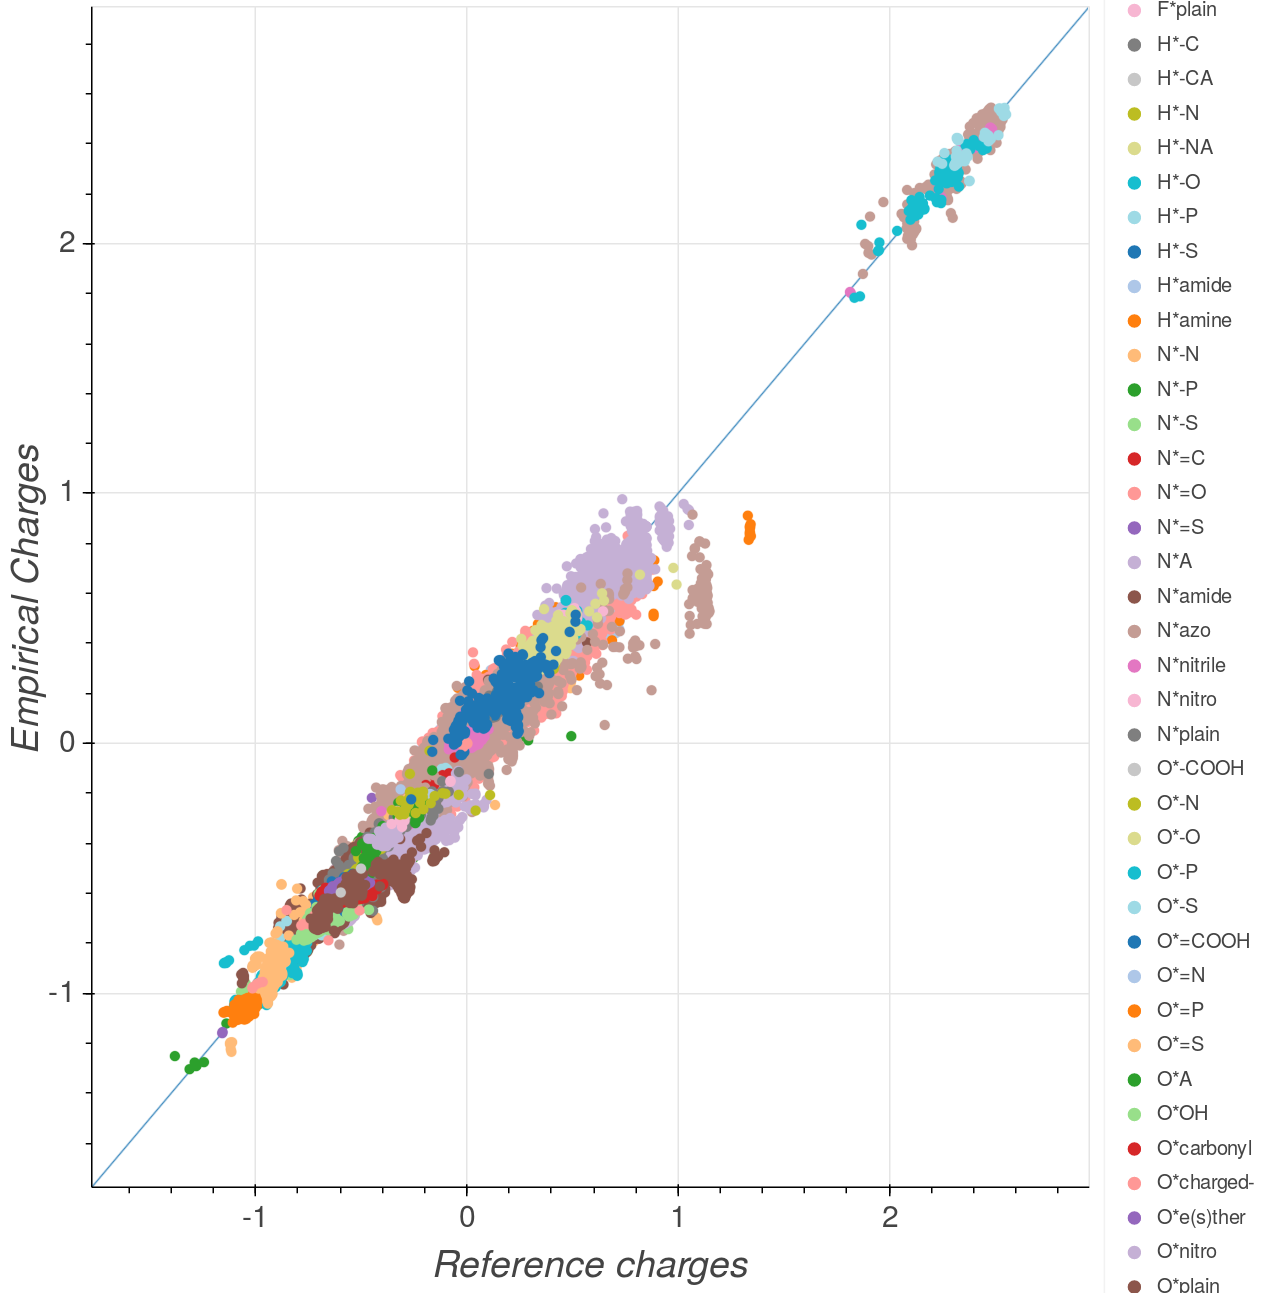
\includegraphics[width=14cm]{pictures/graph_correlation_SDF_EEM_substruct.png}
\caption{Korelační graf parametrizace SDF/EEM/substruct.  PCC$^2$=0,9870; RMSD=0,0479. Legenda ve skutečnosti obsahuje 64 atomových typů, v obrázku je oříznuta na~velikost grafu.}
\label{graph_corr_EEM}
\end{center}
\end{figure}

\begin{figure}[]
\begin{center}
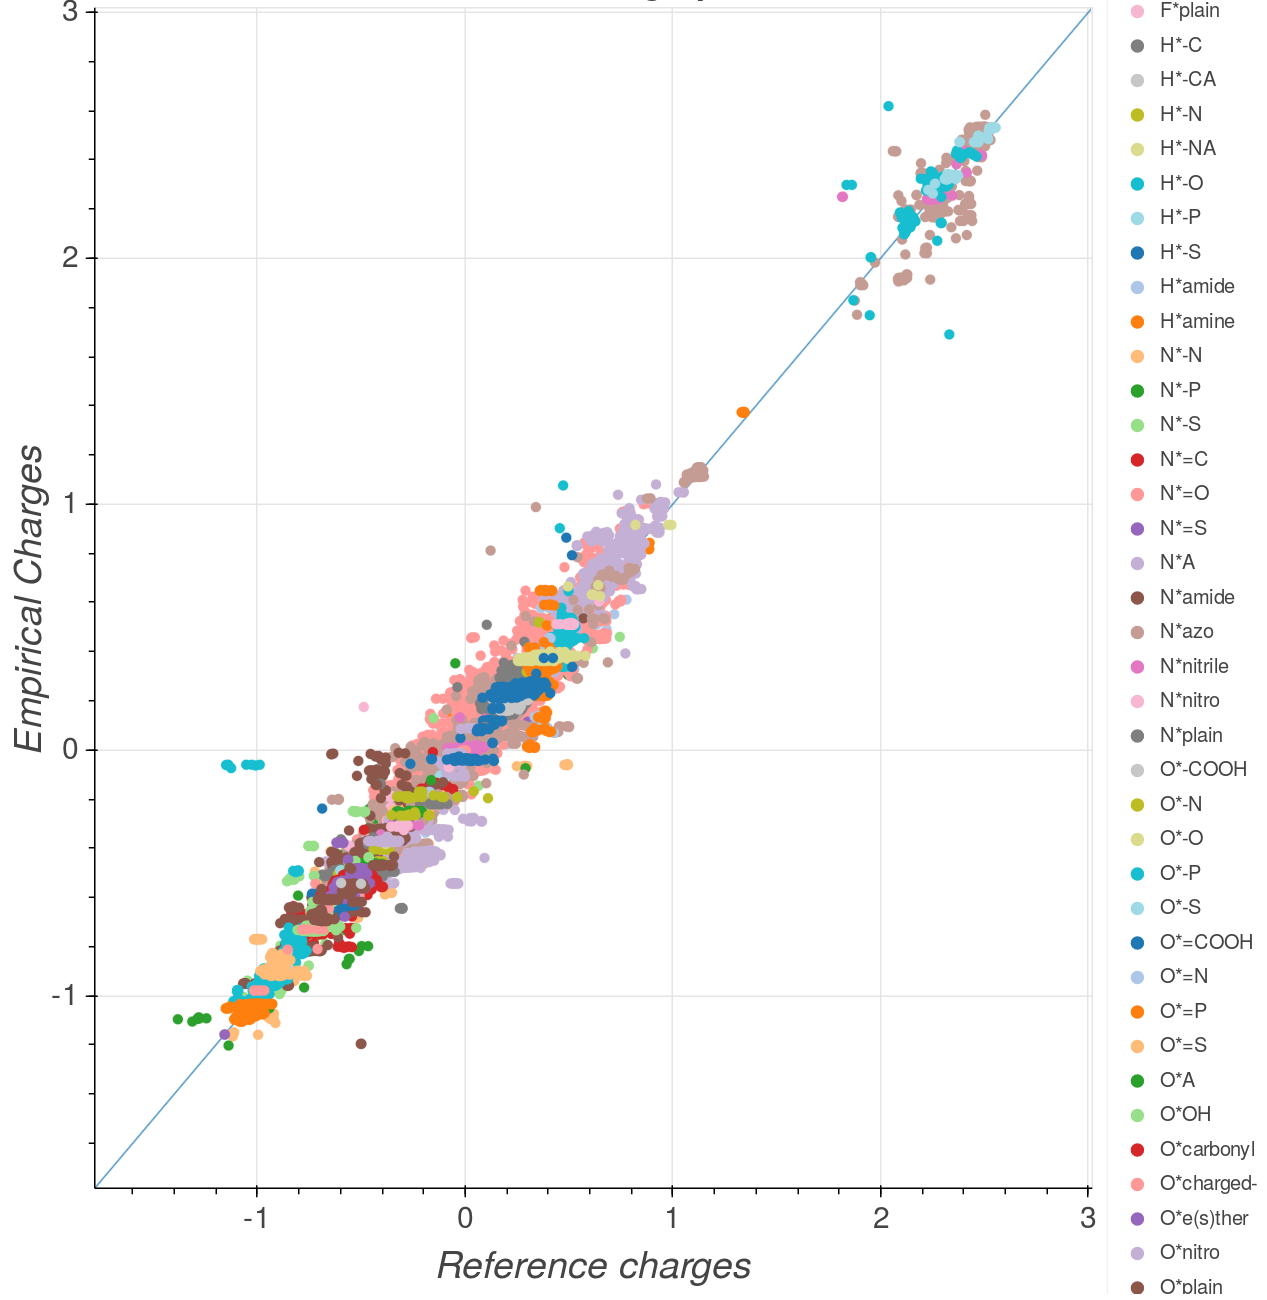
\includegraphics[width=14cm]{pictures/graph_PEOE_substruct.png}
\caption{Korelační graf parametrizace SDF/PEOE/substruct.  PCC$^2$=0,9878; RMSD=0,0464. Legenda ve skutečnosti obsahuje 64 atomových typů, v obrázku je oříznuta na~velikost grafu.}
\label{graph_corr_PEOE}
\end{center}
\end{figure}

\subsection{Statistiky vybraných atomových typů}
Vysoká hodnota PCC$^2$ molekulové sady popisuje míru lineární závislosti hodnot empirických a referenčních nábojů, nevypovídá však o lineární korelaci mezi empirickými a referenčními náboji pro jednotlivé atomové typy.

Pro vybrané atomové typy nabývá PCC$^2$ hodnot blízkých nule, mezi atomy, které jsou daným atomovým typem klasifikované, je tedy detekována nulová lineární závisost mezi empirickými a referenčními náboji. Nízká hodnota kvadrátu Pearsonova korelačního koeficientu vybraného atomového typu může být způsobená přiřazenou konstantní hodnotou empirických nábojů nebo malým počtem atomů, který atomový typ reprezentují. I minimální odchylky nábojů od přímky $y = x$ korelačního grafu se pak projeví do výsledné hodnoty PCC$^2$ atomového typu.
\vspace{0,5cm}
\begin{figure}[h]
\begin{center}
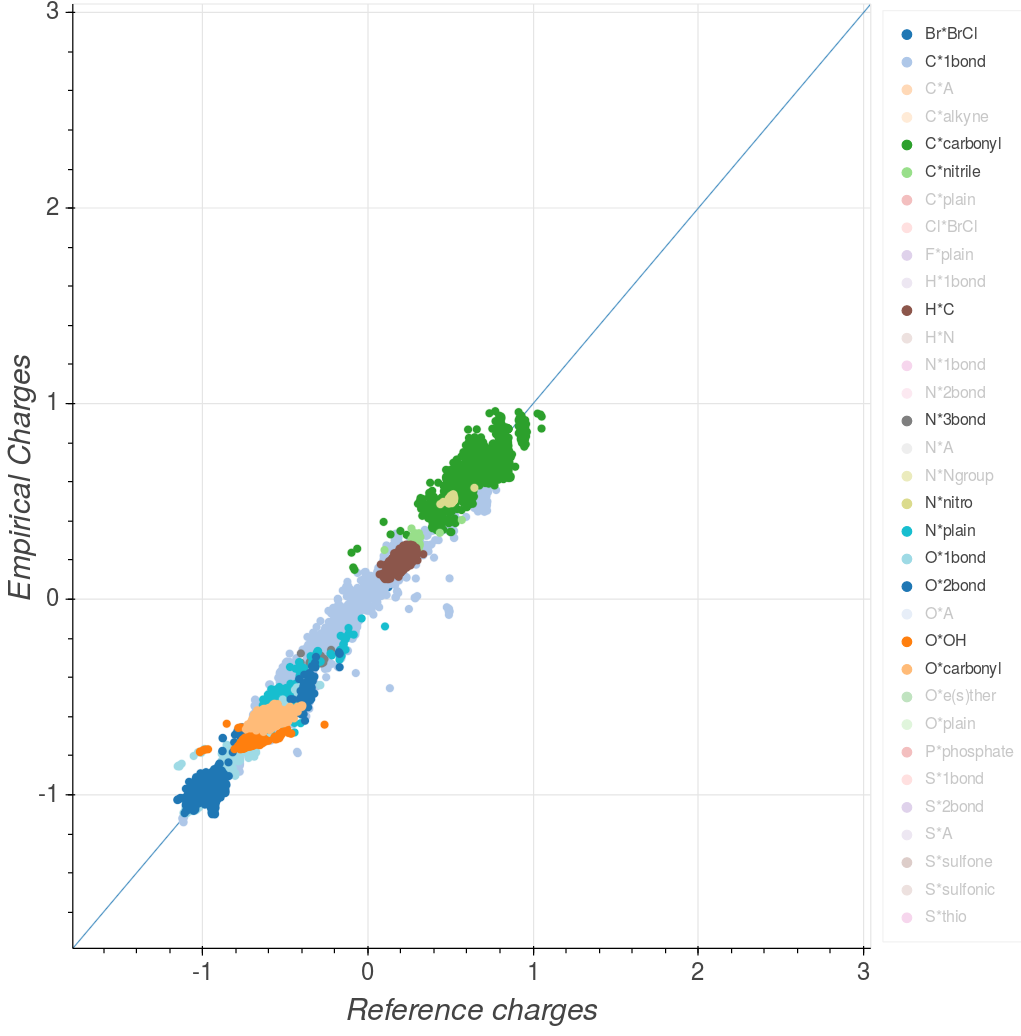
\includegraphics[width=13cm]{pictures/graph_pcc_atom_types.png}
\caption{Korelační graf parametrizace SDF/EEM/substruct\_simplified. PCC$^2$ pro atomové typy 'H*C', 'O*carbonyl' a 'O*OH' nabývá hodnot 0,3702; 0,1501 a 0,3050. Hodnota PCC$^2$ atomového typu 'C*1bond' je 0,9316.}
\label{graph_pcc_atom_types}
\end{center}
\end{figure}

% \begin{figure}[h]
% \begin{center}
% 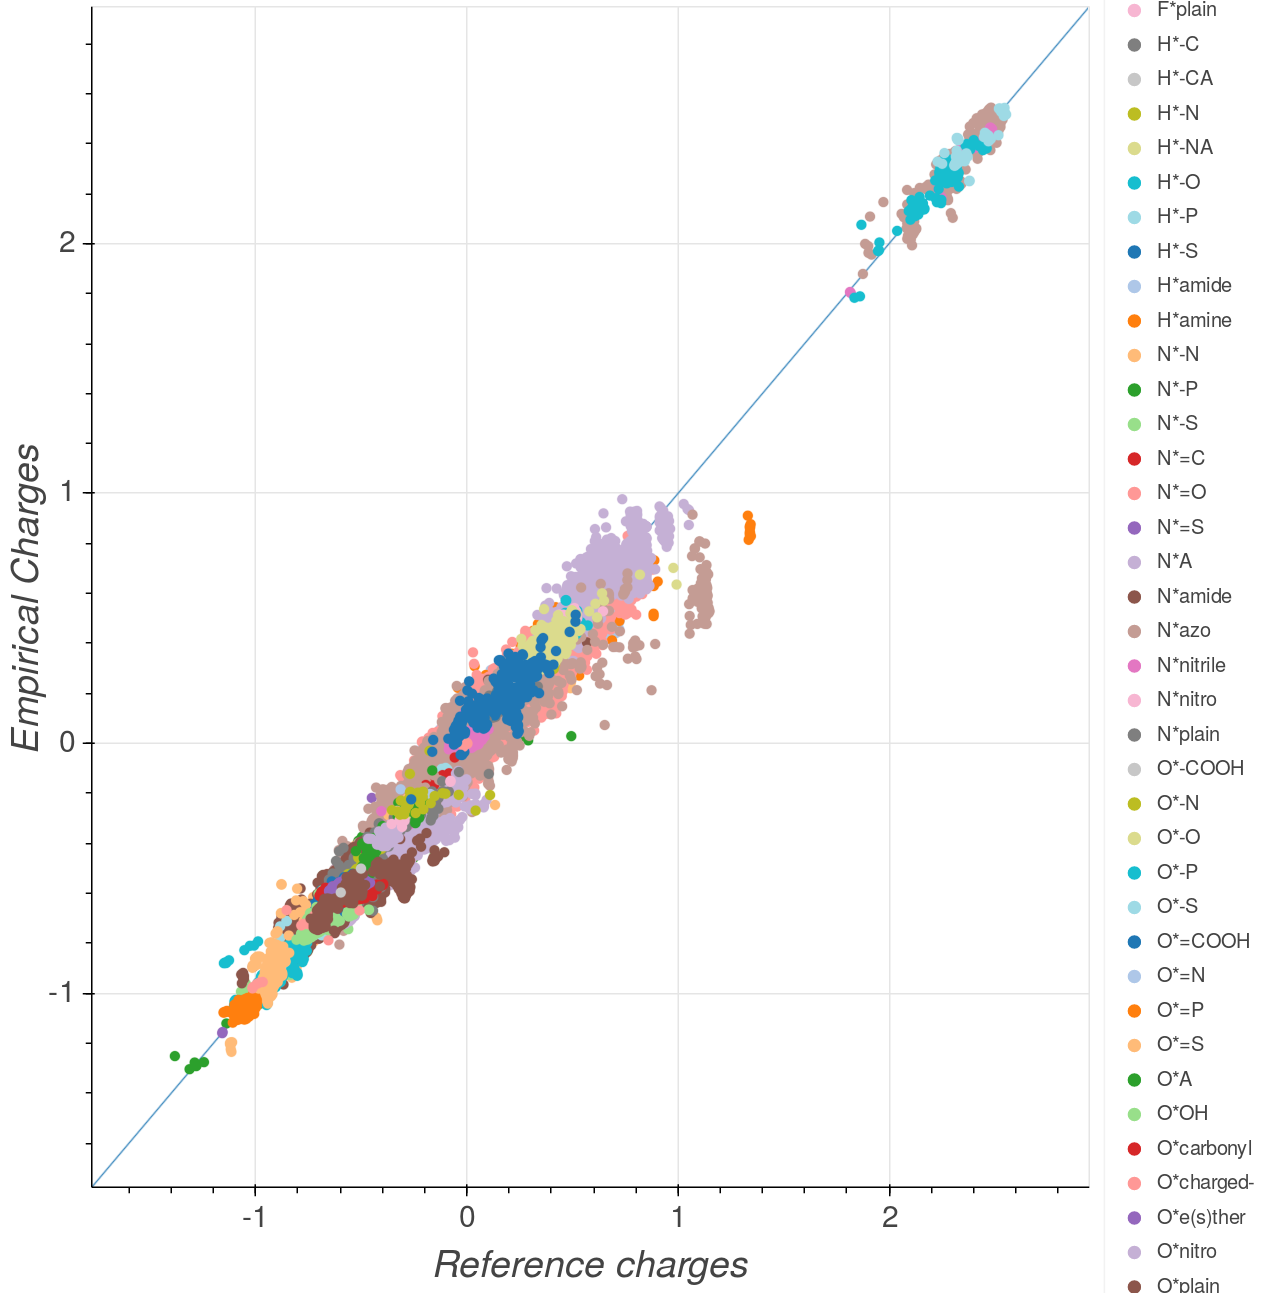
\includegraphics[width=14cm]    {pictures/graph_correlation_SDF_EEM_substruct.png}
% \caption{Korelační graf parametrizace SDF/EEM/substruct.  PCC$^2$=0,9870; RMSD=0,0479. Legenda ve skutečnosti obsahuje 64 atomových typů, v obrázku je oříznuta na~velikost grafu.}
% \label{graph_corr}
% \end{center}
% \end{figure}